% 20200719
\documentclass[../thesis.tex]{subfiles} %% use packages & commands as this main file
\begin{document}
\section{Result}
Biomass densities were stable within days in destructive systems.  \Phy\ biomass densities in both systems dropped during system development (Fig.\ref{f:destCarbon}B).  \Bac\ density had a increase and set back a little to the stable level (Fig.\ref{f:destCarbon}C).  Organic carbon in both systems behaved differently (Fig.\ref{f:destCarbon}A).  It accumulated linearly in \PoN\ but dropped to stability level in \PBN.  Daily yield was significantly different (Fig.\ref{f:ydByHarv}A; p $\ll$ 0.01) between systems or across time except \PoN\ system after the first few days of system development (Fig.\ref{f:ydDaily}A \& \ref{f:ydByHarv}A; p$>$0.1 for \PoN\ day 5 \& 50).  Yield level plateau at long runtime for \phy-only systems but it peaked early in \PBN\ systems (Fig.\ref{f:ydDaily}).  Yet \phy-only systems always had a higher yield distribution than \pbs s with less \phy\ biomass (Fig.\ref{f:destCarbon}B).

Feasible systems in continuous harvest modes had positive yields.  Favourable systems in destructive harvest modes had yields higher than initial values.  100\% \PoH\ (n=5500, N=5500; $x$=19500 \dayU; IQR=[0.039, 1.853] \dxdt; median=0.371 \dxdt; max=346 \dxdt) and 0.3\% \PBH\ (n=19; $x$=2101 \dayU; IQR=[12.4, 47.8] \dxdt; median=25.2 \dxdt; max=285 \dxdt) systems were feasible.  100\% \PoN\ (n=5500; $T$=19900 days; IQR=[0.045, 1.851] \dxdt; median=0.379 \dxdt; max=346 \dxdt) and 97.2\% \PBN\ (n=5346; $T$=91 days; IQR=[-0.012, 0.141] \dxdt; median=0.019 \dxdt; max=243 \dxdt) systems were favourable.  Most system pairs showed significance in median difference (\PoH\ vs \PoN: p=0.36; other pairs: p$\ll$0.01).  \Bac l invasion into \PoN\ systems would largely reduce its expected yield (Fig.\ref{f:bacEffect}).  With the right combination of \phy\ and \bac, \pbs s could also have yield comparable with \phy-only systems.

Most \phy\ biology had significant (p$\ll$0.01 for Wilcox test across the ends of parameter ranges) unidirectional ($\ePR$, $\eP$, $\gP$: positive; $\aP$: negative) effect on log yield distributions (Fig.\ref{f:bacEffect}).  \Bac\ biology had no observable distribution influences (Fig.\ref{f:bacEffect2}).  Harvest modes determined feasibility of \pbs s (Fig.\ref{f:harvPB}) but had no effect on \phy-only systems (Fig.\ref{f:harvPo}).  In short, yield distribution maximized when \phy\ had high carbon-to-biomass ratio (high $\ePR$ and $\eP$), high growth rate (high $\gP$) and low intraspecific interference (low $\aP$).

\begin{figure}[H]
    \centering
    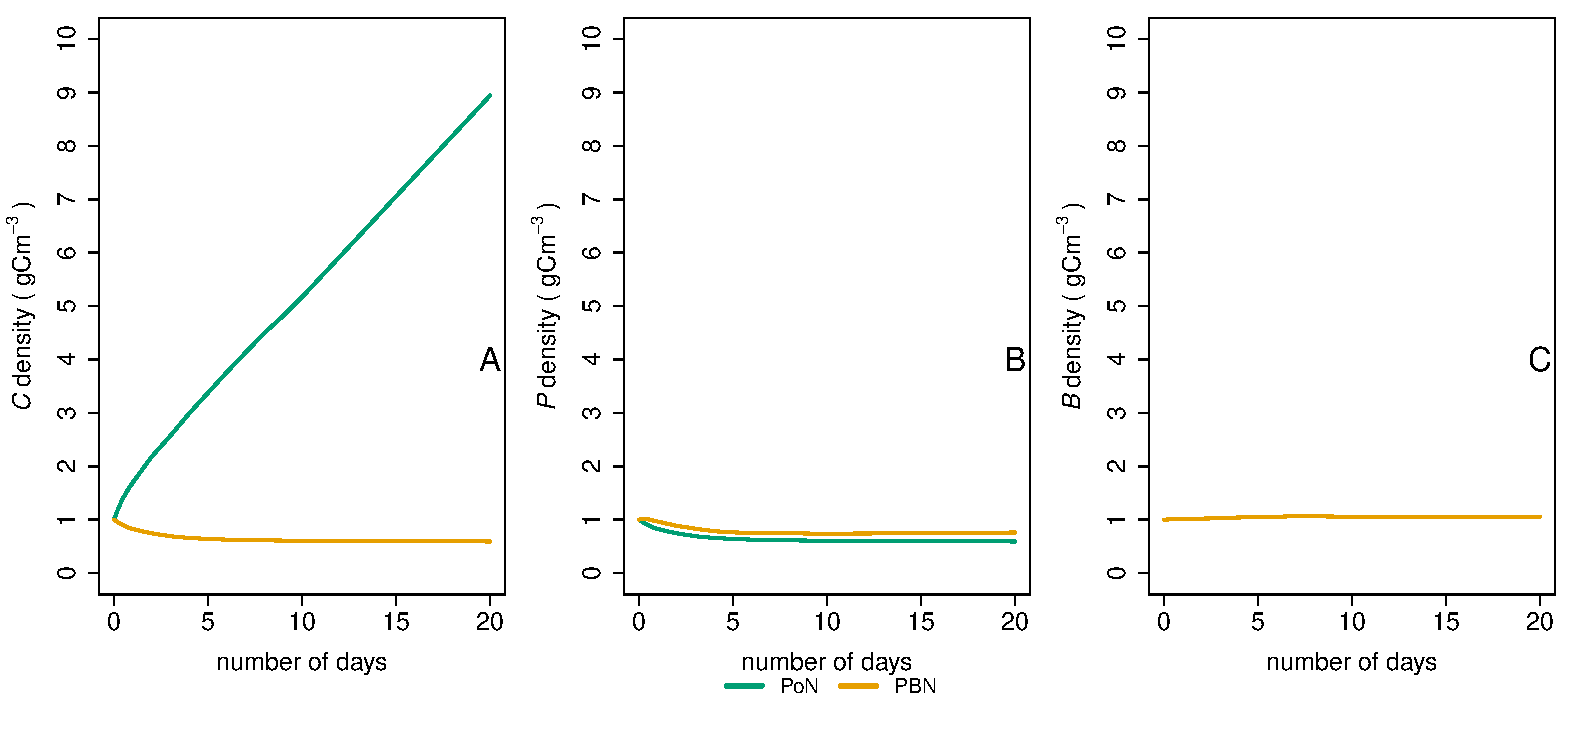
\includegraphics[width=\linewidth]{result/Sample.pdf}
    \caption[Median carbon content in destructive systems]{Median carbon content in destructive systems.  $C$, $P$ and $B$ were carbon pools in Fig.\ref{f:model}.  Eq.\ref{eq:PBH} was used with different initial carbon densities to address the \PoN\ and \PBN\ modes.  Initial carbon densities for \PoN\ were [1,1,0]\den\ ($C$, $P$, $B$) and that for \PBN\ were [1,1,1]\den.  Note that both systems had similar levels of \phy\ across time \textbf{(B)}.  Yet due to the presence of \bac\ \textbf{(C)}, organic carbon pool density changes were huge \textbf{(A)}.  Also note that after a initial boost, accumulation of organic carbon was linear for \PoN\ \textbf{(A)}.  Note that existence of \bac\ suppressed the organic carbon density in the system \textbf{(A)} with almost unchanged \bac\ biomass density \textbf{(C)}.}
    \label{f:destCarbon}
\end{figure}

\begin{figure}[H]
    \centering
    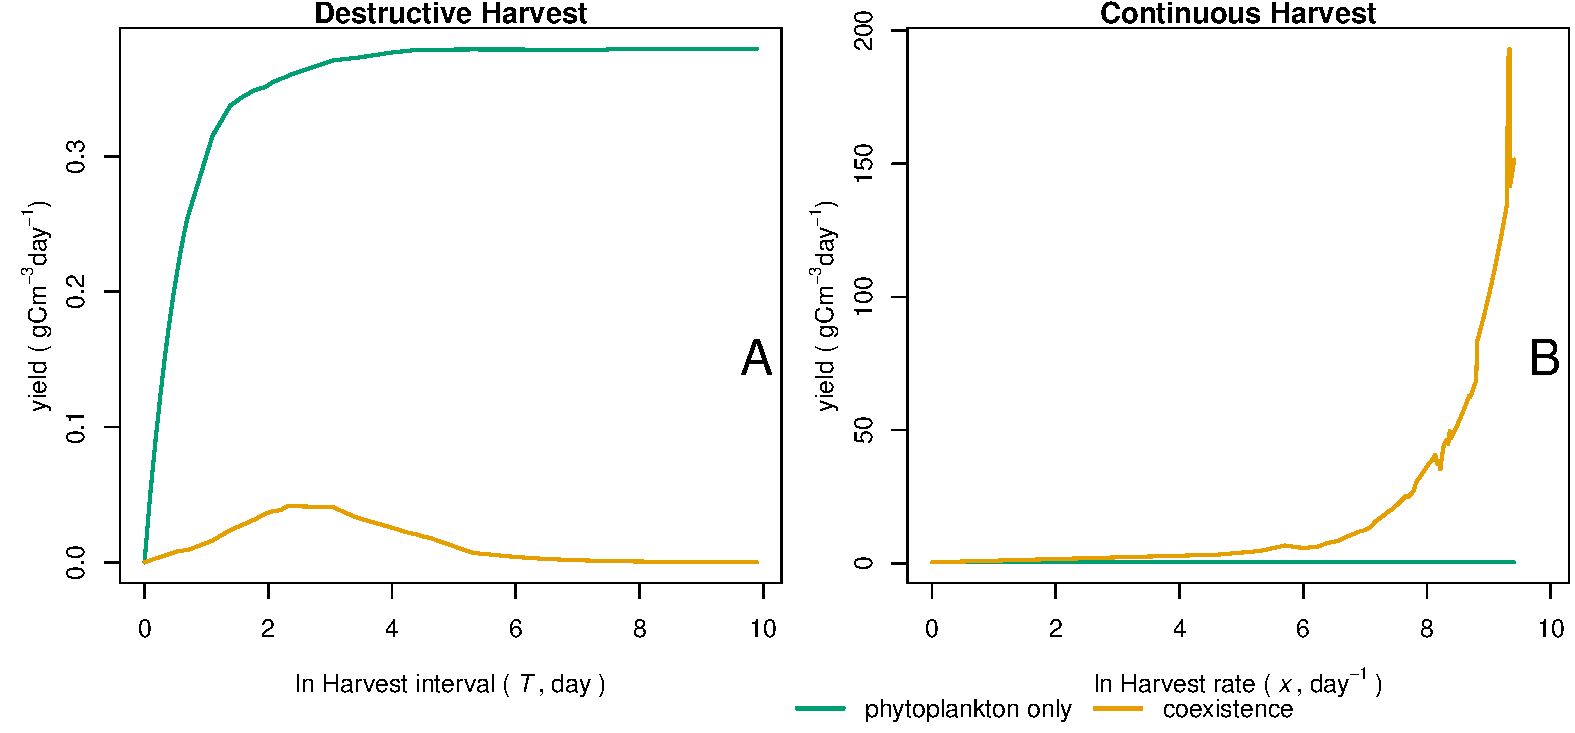
\includegraphics[width=\linewidth]{result/DailyYield.pdf}
    \caption[Median daily yield across systems]{Median daily yield across systems.  Note that both harvest interval/rate were natural logged.  In \textbf{A}, the minimal optimum harvest interval for \PoN\ was around 3 days (i.e. exp(1)) while peak yield achieved at day 20 (i.e. exp(3)) for \PBN.  In \textbf{(B)}, very high daily harvest escalated output of \PBH\ systems.  Yet the \PBH\ median represents only the 0.3\% (n=19) feasible systems out of 5500 scenarios.}
    \label{f:ydDaily}
\end{figure}

\begin{figure}[H]
    \centering
    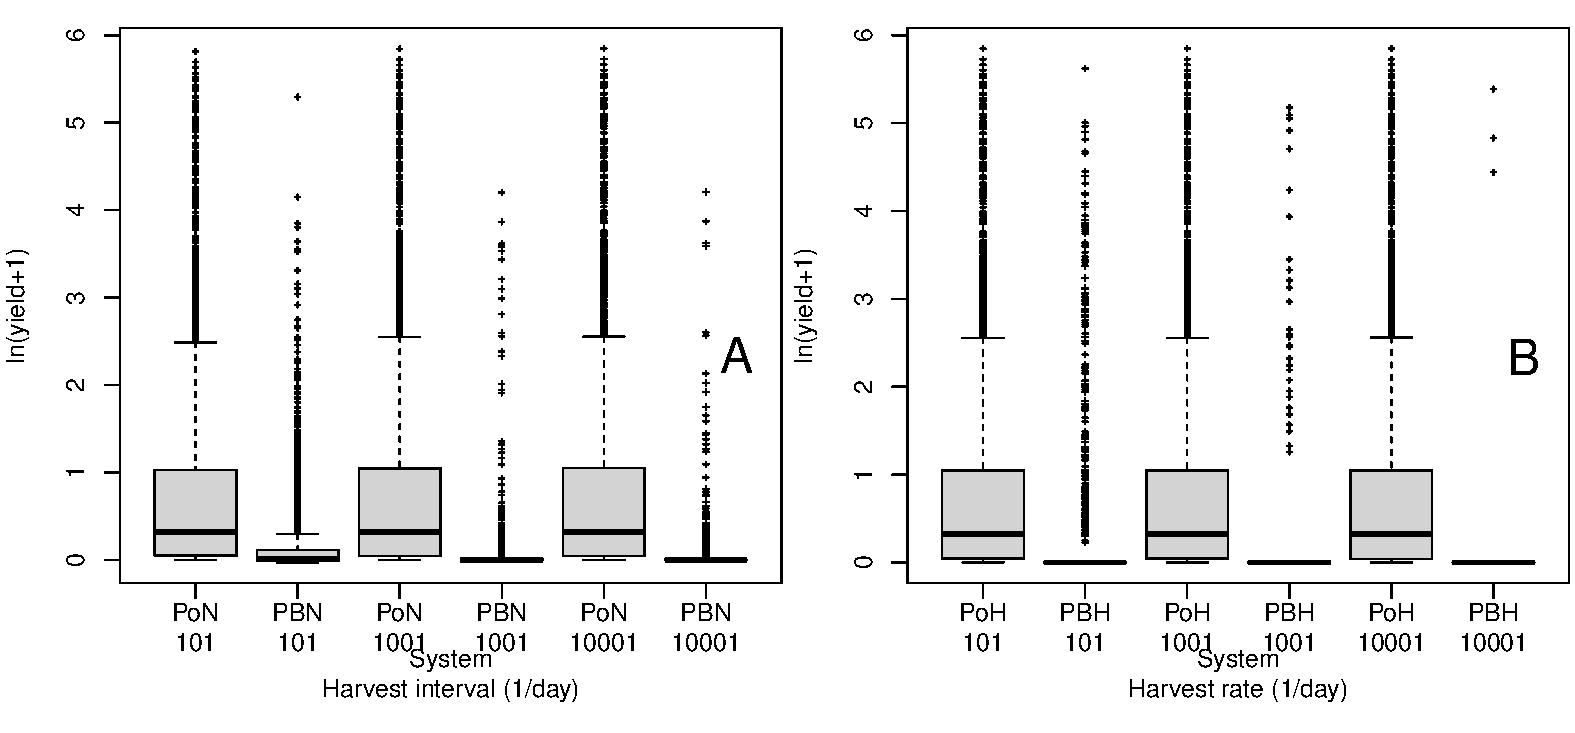
\includegraphics[width=\linewidth]{result/Harvest.pdf}
    \caption[Yield flux distribution by harvest mode]{Log distribution of feasible scenarios on selected harvest interval/rates.  \textbf{(A)}  Note that log yield distributions for \PoN\ between day 5 and 50 were non-significant in median (p$>$0.1).  All boxes had a sample size of 5500 except \PBN, n=5454.  Some \PBN\ systems had an initial drop of carbon content (day 0.5) but all recovered within a few days.  \textbf{(B)} Note that each \PoH\ log yield distribution had 5500 scenarios.  Distributions were non-significant between rates (p $>$ 0.1).  Note that only feasible \PBN\ systems were recorded, which the boxes represented 184 ($x$=100 \dayU), 31 ($x$=1000 \dayU) and 3 ($x$=10K \dayU) scenarios out of 5500.}
    \label{f:ydByHarv}
\end{figure}

\begin{figure}[H]
    \centering
    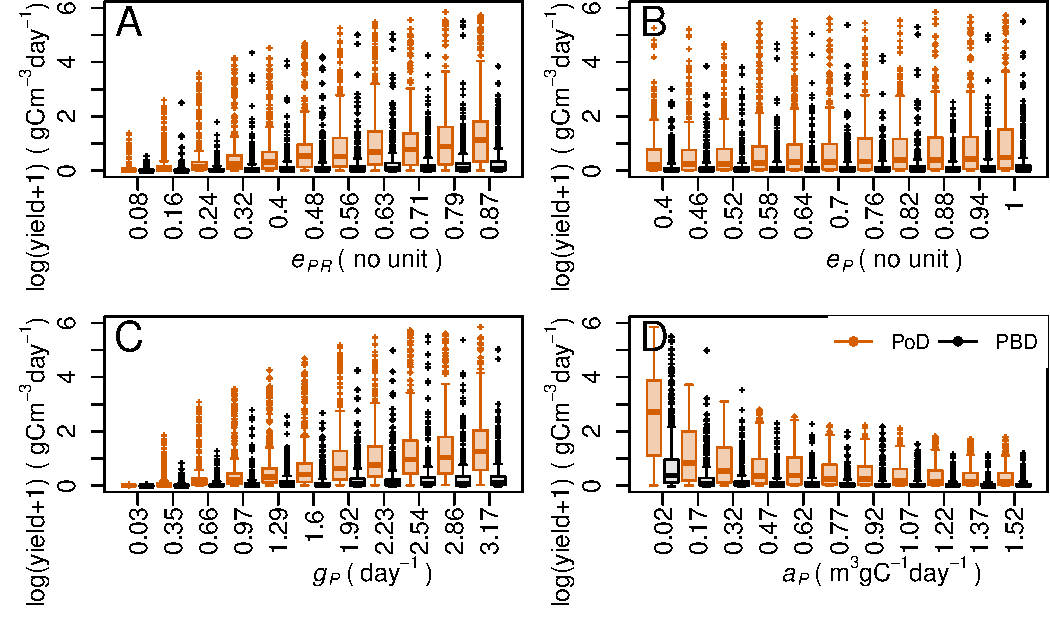
\includegraphics[width=\linewidth]{result/bacEff1.pdf}
    \caption[Log yield flux comparisons between \phy-only and \pbs s on \phy\ parameters]{Log yield flux comparisons between \phy-only and \pbs s on \phy\ parameters.  Full description of variables were in Table \ref{t:ranges}.  Each group in each plot had an LHS sample size of 5500.  Pairwise Wilcox test showed significance (all p $\ll$ 0.01) between the systems and the ends of parameter ranges.  Note that ranges of both groups were similar, symbolising comparable yield values were possible for \pbs s.}
    \label{f:bacEffect}
\end{figure}

\begin{figure}[H]
    \centering
    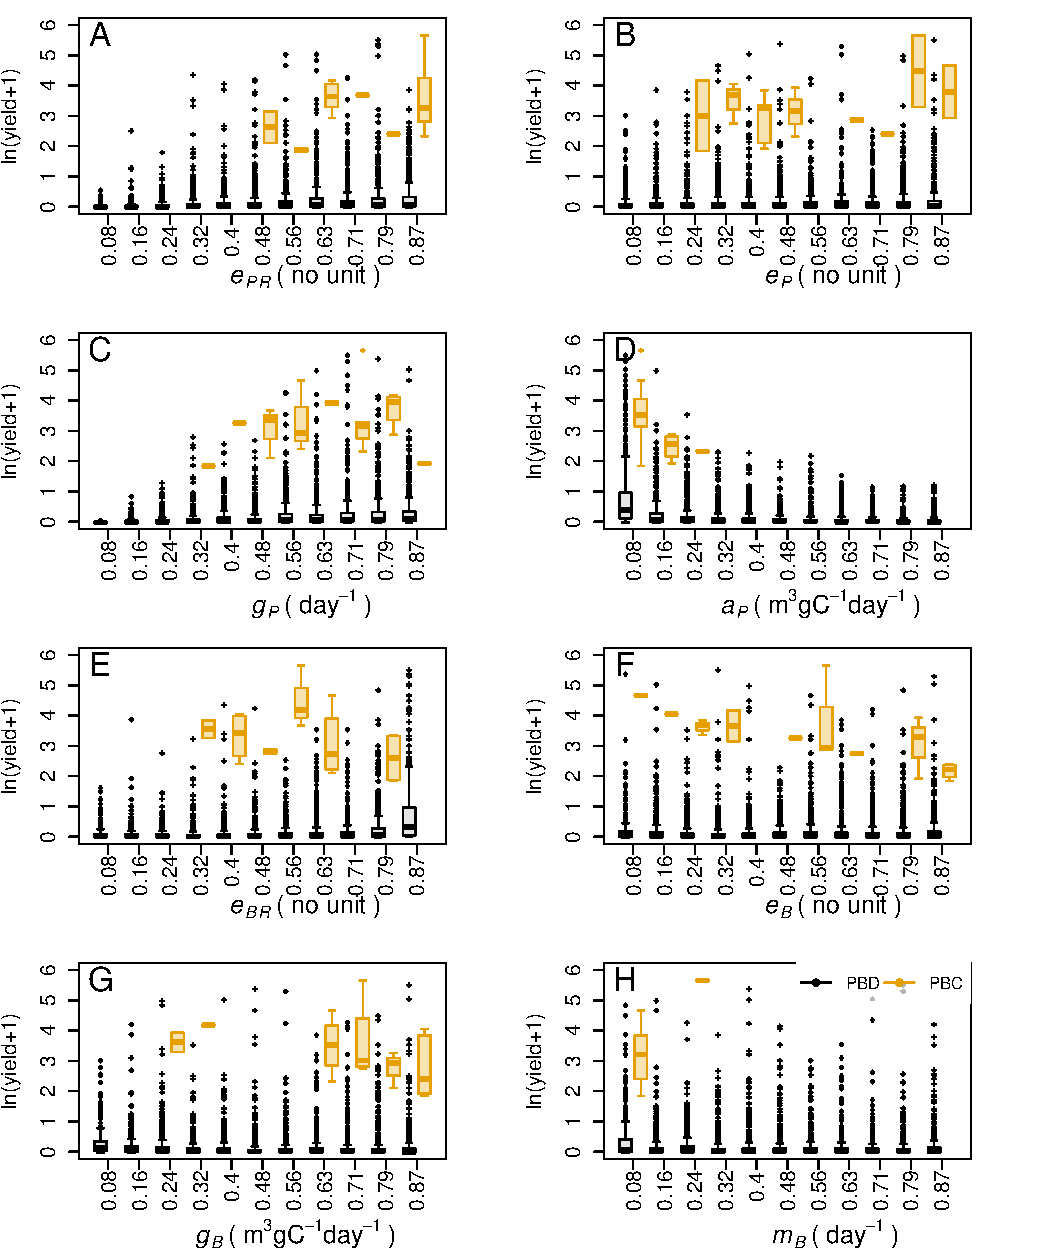
\includegraphics[width=\linewidth]{result/harvB.pdf}
    \caption[Log yield flux comparisons between \pbs s]{Log yield flux comparisons between \pbs s.  For each independent variable value, the box on its left represented \PBN\ while the one on the right represented \PBH.  Full description of variables were in Table \ref{t:ranges}.  Each group in each plot had an LHS sample size of 5500.  Pairwise Wilcox test showed significance (p $\ll$ 0.01) between the systems.  Note that only a few scenarios of \pbs s were positives, which symbolised small feasibility.  Also note that the highest value of \PBH\ was higher than that of \PBN\ systems, indicating the best scenario of continuous harvest systems yielded higher than that of \PBN.  Yet \PBN\ systems had more feasible scenarios (97.2\%) than \PBH\ ones (0.3\%).}
    \label{f:harvPB}
\end{figure}

\end{document}